
\begin{tikzpicture}[every node/.style={scale=1.0}] 
	\node[anchor=south west,inner sep=0] (image) at (0,0) {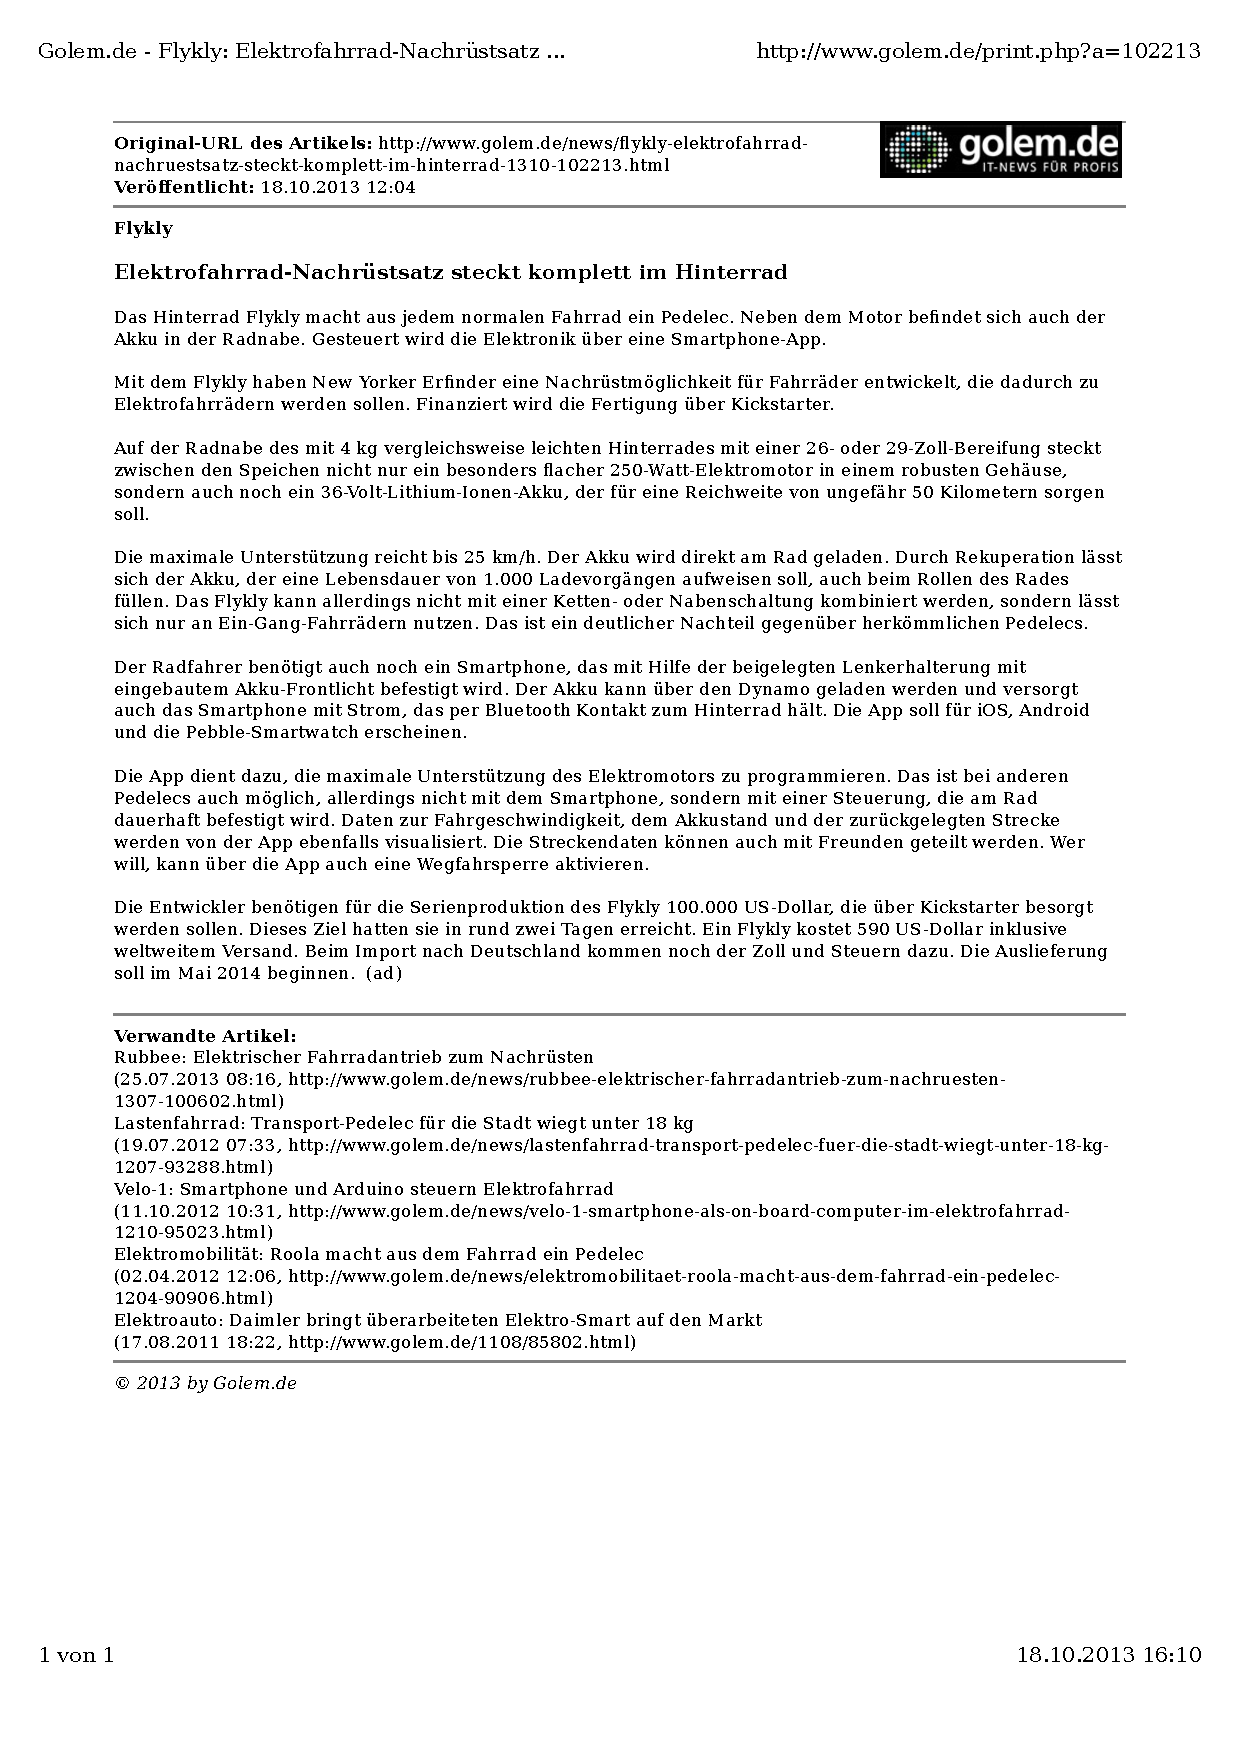
\includegraphics[trim=1.8cm 13cm 2cm 2.0cm,clip]{\dir/zeitungsartikel_e-velo.pdf}};
	%% trim= 1 2 3 4 `crops’ the picture by 1bp at the left, 2bp at the bottom, 3bp on the right and 4bp at the top.
\end{tikzpicture} 

\begin{aufgabe}
	\begin{enumerate} [a)]
		\item	Lesen Sie den Zeitungsartikel und beschreiben Sie in zwei Sätzen worum es darin geht.
			\TAX{Text K1}
		\item Berechnen Sie den Rollwiderstand $\RI{F}{Roll}$ für ein \SI{20}{kg} schweres Velo.
			Die Masse des Fahrers soll \SI{60}{kg} betragen.
			Nehmen Sie einen Rollwiderstandsbeiwert von $c=0.01$ an.
			\TAX{Berechnung mit numerischem Resultat K2}
		\item Berechnen Sie den Luftwiderstand bei einer Geschwindigkeit von \SI{20}{km/h}. Die effektive
			Stirnfläche $c_w\cdot A$ soll $\num{0.75}$ sein.
			\TAX{Berechnung mit numerischem Resultat K2}
		\item Zeichnen Sie die Geschwindigkeits-Leistungs-Diagramm. Welche maximale Geschwindigkeit ist demnach mit dem Velo möglich?
			\TAX{Graphische Darstellung K2}
		\item Ist es möglich die \SI{30}{km} von Bern (542\ m\ ü.\ M.) nach Thun (560\ m\ ü.\ M.) ausschliesslich im Elektrobetrieb zurückzulegen?
			Wenn ja, wie lange dauert die Fahrt mindestens?
			\TAX{Qualitative Abschätzung K3}
	\end{enumerate}
\end{aufgabe}
